\section{Propietats de les sèries temporals}

En el model de \gls{SGST} descrit anteriorment, les sèries temporals
tenen una única estructura i uns únics operadors independentment del
context on s'apliquin. De fet aquest és l'objectiu principal de
definir-ne un model lògic. No obstant això, en la seva aplicació les
sèries temporals tenen associat un context, és a dir que els valors
prenen un determinat significat. En aquesta secció avaluem les
propietats que poden prendre les sèries temporals quan es troben en
context:
\begin{itemize}
\item Trets semàntics: el significat que tenen en
  el seu àmbit d'aplicació
\item Grafs i representacions: les visualitzacions i interpretacions
  possibles
\item Patologies: els casos problemàtics de les sèries temporals
\end{itemize}




\subsection{Trets semàntics de les sèries temporals}

Una sèrie temporal pot provenir de varis àmbits i per tant tenir un
significat variat. És el que anomenem trets semàntics de les sèries
temporals.


En el model d'operacions s'ha vist que l'atribut de temps de les
sèries temporals indueix vàries naturaleses en el comportament dels
operadors: com a conjunts, com a seqüències o com a funcions
temporals. Aquesta distinció de significat és des del punt de
vista de formalització matemàtica per l'estructura de les sèries
temporals.

A continuació distingim el significat de les sèries temporals segons
l'origen; és a dir com s'han adquirit o de quin entorn
provenen. Aquesta distinció és important per a determinar quines
operacions tenen sentit de ser aplicades i quines no a una sèrie
temporal en particular. Així \textcite{segev87:sigmod} anomenen
comportament semàntic (\emph{semantic behavior}) a la varietat de
formes que pot prendre una sèrie temporal segons l'àmbit on
s'apliquen.


\subsubsection{Aparell de mesura}

Un primer tret semàntic de les sèries temporals és deu al mètode
d'adquisició segons l'aparell de mesura. Així una sèrie temporal es
pot classificar segons si s'ha adquirit mostrejant un senyal continu
cada cert període o si prové d'una acumulació o d'un comptatge
d'esdeveniments en un cert període de temps. Aquests són els dos
orígens principals que poden tenir els senyals discrets segons
\textcite[cap.~1]{proakismanolakis96}.  En aquest tret es distingeix
segons l'adquisició en l'eix del temps, també es pot distingir segons
si l'adquisició en l'eix de valors és contínua o discreta però això és
un tret propi dels valors i, com a característica, pertany al domini
dels valors. Aquest procés en l'eix de valors s'anomena quantització
del senyal però sovint, per simplificar, no es té en
compte \parencite{proakismanolakis96}.%S1.4.7



Així doncs segons l'aparell de mesura, classifiquem una sèrie
temporal amb trets de magnitud física o de comptador de magnitud
física. Aquest tret semàntic cal tenir-lo en compte ja que quan
s'adquireix una magnitud es veu el seu estat instantani actual, mentre
que quan s'adquireix un comptador ofereix informació de la seva
variació respecte a l'adquisició anterior.



\begin{figure}[tp]
  \centering
    \begin{tabular}[c]{|c|c|}
    \multicolumn{2}{c}{$S_m$} \\ \hline
    $t$  & $v$ \\ \hline
    0   & 0 \\
    2   & 1 \\
    3   & 1{,}5 \\
    4   & 0 \\
    5   & 2 \\ 
    8   & 2 \\ \hline
  \end{tabular} \qquad
  \begin{tikzpicture}[baseline=(current bounding box.center)]
    \begin{axis}[
        timeseriesrel,
        title=$S_m$,
        ]
    \addplot[blue] coordinates {
        (0,0)
        (2,1)
        (3,1.5)
        (4,0)
        (5,2)
        (8,2)
    };
    %\addlegendentry{Valor absolut}
    \addplot[only marks,mark=*,red] coordinates {
        (0,0)
        (2,1)
        (3,1.5)
        (4,0)
        (5,2)
        (8,2)
    };
    % \addlegendentry{Punts de mesura}
    \end{axis}
  \end{tikzpicture}
 

  \caption{Magnitud física}
  \label{fig:model:magnitud}
\end{figure}

\begin{figure}[tp]
  \centering
    \begin{subfigure}{\textwidth}
    \centering
  \begin{tabular}[c]{|c|c|}
    \multicolumn{2}{c}{$S_a$} \\ \hline
    $t$  & $v$ \\ \hline
    0   & 0 \\
    2   & 1 \\
    4   & 3 \\
    5   & 4 \\
    8   & 10 \\ \hline
  \end{tabular} \qquad
  \begin{tabular}[c]{|c|c|}
    \multicolumn{2}{c}{$S_\Delta$} \\ \hline
    $t$  & $v$ \\ \hline
    0   & 0 \\
    2 & 1 \\
    4 & 2 \\
    5 & 1 \\
    8 & 6 \\ \hline
  \end{tabular} \qquad
  \begin{tabular}[c]{|c|c|}
    \multicolumn{2}{c}{$S_v$} \\ \hline
    $t$  & $v$ \\ \hline
    0   & 0 \\
    2 & 0{,}5 \\
    4 & 1 \\
    5 & 1 \\
    8 & 2 \\ \hline
  \end{tabular}
  \caption{Taules de valors}
  \end{subfigure}

  \begin{subfigure}{0.3\textwidth}
  \begin{tikzpicture}
    \begin{axis}[
        timeseriesrel,
        title=$S_a$,
        ]
    \addplot[blue] coordinates {
        (0,0)
        (2,1)
        (4,3)
        (5,4)
        (8,10)
    };
    %\addlegendentry{Valor absolut}
    \addplot[only marks,mark=*,red] coordinates {
        (0,0)
        (2,1)
        (4,3)
        (5,4)
        (8,10)
    };
    % \addlegendentry{Punts de mesura}
    \end{axis}
  \end{tikzpicture}
  \caption{Valor absolut}
    \label{fig:model:comptador-formes:absolut}
  \end{subfigure}
  \begin{subfigure}{0.3\textwidth}
  \begin{tikzpicture}
    \begin{axis}[
        timeseriesrel,
        title=$S_\Delta$,
        ]
    \addplot[ycomb,blue,mark=-] coordinates {
        (0,0)
        (2,1)
        (4,2)
        (5,1)
        (8,6)
    };
    %\addlegendentry{Increments}
    \addplot[only marks,mark=*,red] coordinates {
        (0,0)
        (2,1)
        (4,2)
        (5,1)
        (8,6)
    };
    %\addlegendentry{Punts de mesura}

    \addplot[gray,dashed] coordinates {
        (0,0)
        (2,1)
        (4,2)
        (5,1)
        (8,6)
    };
    % \addlegendentry{Tendència}

    \end{axis}
  \end{tikzpicture}
  \caption{Increments}
  \label{fig:model:comptador-formes:increments}
  \end{subfigure}
 \begin{subfigure}{0.3\textwidth}
  \centering
  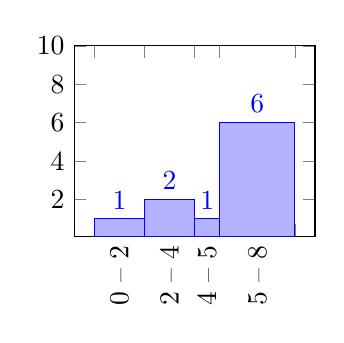
\begin{tikzpicture}
    \begin{axis}[
%        timeseriesrel,
        height=4cm,
        %width=10cm,scale only axis, height=5cm,
        ymax = 10,
        xtick = data,
        xticklabel interval boundaries,
        x tick label style= {rotate=90,anchor=east},
        x label style ={ at={(1,0)},left,yshift=0pt},
        ]
    \addplot[ybar interval,blue,fill=blue!30!white] coordinates{
        (0,1)
        (2,2)
        (4,1)
        (5,6)
        (8,6)
    }; 
    % \addlegendentry{Increments}

    \node[color=blue,above] at (axis cs:1,1) {1};
    \node[color=blue,above] at (axis cs:3,2) {2};
    \node[color=blue,above] at (axis cs:4.5,1) {1};
    \node[color=blue,above] at (axis cs:6.5,6) {6};
    \end{axis}
  \end{tikzpicture}
  \caption{Gràfic de barres}
    \label{fig:model:comptador-formes:barres}
  \end{subfigure}

  \begin{subfigure}{0.3\textwidth}
  \centering
  \begin{tikzpicture}
    \begin{axis}[
        timeseriesrel,
        title=$S_\Delta$
        ]
    \addplot[blue] coordinates {
        (0,0)
        (2,1)
        (2,0)
        (4,2)
        (4,0)
        (5,1)
        (5,0)
        (8,6)
        (8,0)
    };
    %\addlegendentry{Valor relatiu}
    \addplot[only marks,mark=*,red] coordinates {
        (0,0)
        (2,1)
        (4,2)
        (5,1)
        (8,6)
    };
    %\addlegendentry{Punts de mesura}
    \end{axis}
  \end{tikzpicture}
  \caption{Valor relatiu}
    \label{fig:model:comptador-formes:relatiu}
  \end{subfigure}
  \begin{subfigure}{0.3\textwidth}
  \centering
  \begin{tikzpicture}
    \begin{axis}[
        timeseriesrel,
        title=$S_v$,
        ymax=2.3,
        ]
    \addplot[const plot mark right,blue] coordinates {
        (0,0)
        (2,0.5)
        (4,1)
        (5,1)
        (8,2)
    };
    %\addlegendentry{Velocitat mitjana}

   \addplot[only marks,mark=*,red] coordinates {
        (0,0)
        (2,0.5)
        (4,1)
        (5,1)
        (8,2)
    };
    %\addlegendentry{Punts de mesura}

    \end{axis}
  \end{tikzpicture}
  \caption{Velocitat}
    \label{fig:model:comptador-formes:velocitat}
   \end{subfigure}
  \begin{subfigure}{0.3\textwidth}
  \centering
  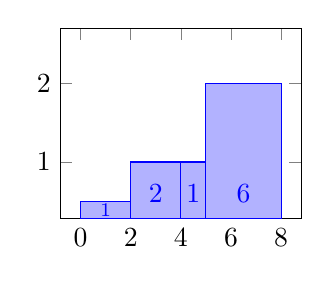
\begin{tikzpicture}
    \begin{axis}[
        height=4cm,
        ymax=2.7,
        ]
    \addplot[ybar interval,blue,fill=blue!30!white,mark=none] coordinates {
        (0,0.5)
        (2,1)
        (4,1)
        (5,2)
        (8,2)
    };
    %\addlegendentry{distribució d'increments}

    \node[color=blue] at (axis cs:1,0.39) {\scriptsize 1};
    \node[color=blue] at (axis cs:3,0.6) {2};
    \node[color=blue] at (axis cs:4.5,0.6) {1};
    \node[color=blue] at (axis cs:6.5,0.6) {6};
     \end{axis}
  \end{tikzpicture}
  \caption{Histograma}
  \label{fig:model:comptador-formes:histograma}
  \end{subfigure}

  \caption{Formes d'un comptador monòton}
  \label{fig:model:comptador-formes}
\end{figure}



Les magnituds ofereixen la informació d'una forma: l'estat de la
variable. A la \autoref{fig:model:magnitud} es mostra aquesta forma
amb una sèrie temporal d'exemple: $S_a = \{(0,0),(2,1),(3,
1{,}5),(4,0),(5,2),(8,2)\}$. De manera general, el valor d’una
magnitud física és defineix com el producte d’un valor numèric per una
unitat.


Els comptadors poden oferir la informació de diverses formes : en
valor absolut, en valor relatiu i en velocitat. A la
\autoref{fig:model:comptador-formes} es mostren aquestes formes amb
tres sèries temporals d'exemple: $S_a =
\{(0,0),(2,1),(4,3),(5,4),(8,10)\}$ són els valors absoluts del
comptador, $S_\Delta = \{(0,0)\} \cup
\glssymbol{not:sgst:increments}(S_a) =
\{(0,0),(2,1),(4,2),(5,1),(8,6)\}$ són els valors relatius del
comptador i $S_v = S_\Delta /
\glssymbol{not:sgst:increments}(\glssymbol{not:sgst:duplica-t}(S_\Delta))
= \{(0,0),(2,0{,}5),(4,1),(5,1),(8,2)\}$ són els valors de velocitat
del comptador, les unitats dels quals són de \emph{unitat$/$unitat de
  temps}.


El gràfic de valor absolut, en aquest cas es tracta d'un comptador
monòton creixent, mostra la interpolació lineal del valor acumulat que
va prenent la variable mesurada. A partir del valor absolut es poden
calcular els increments del comptador, és a dir la quantitat relativa
de cada període. En el gràfic d'increments es mostra en línia
discontínua la tendència dels increments, és a dir la interpolació
lineal del comptatge absolut com si el comptador fos una
magnitud, que cal no confondre amb el gràfic de valor relatiu que
mostra la interpolació lineal que va prenent la variable mesurada
relativament, és a dir amb el pas per zero com si a cada lectura
s'inicialitza de nou el valor acumulat del comptador. El gràfic de
velocitat mostra els pendents lineals del gràfic de valor relatiu, és
a dir la velocitat mitjana de comptatge a cada període.

El significat del gràfic de valor absolut i el d'increments es
visualitza bé en un gràfic de barres en el que l'eix vertical mostra
freqüència i en el que l'alçària de les barres mostra la quantitat que
ha augmentat el comptador a cada interval. En canvi el gràfic de valor
relatiu i el de velocitat es visualitzen més bé en un gràfic
d'histograma en el que l'eix vertical mostra densitat de freqüència i en el
que l'àrea de les barres equival a la quantitat comptada i l'alçària
de cada una mostra la velocitat del comptatge.


En conclusió, un comptador pot oferir les dades en qualsevol de les
tres formes i a partir d'una d'aquestes es poden calcular les
altres. També es possible d'aplicar les mateixes operacions a les
magnituds, és a dir calcular-ne els increments o la velocitat mitjana
de cada període, tenint en compte que aleshores es perd la referència
absoluta llevat que es conservi a part. La diferència principal
d'ambdós rau en el fet que l'objectiu de les magnituds és observar el
valor instantani d'una variable i per tant se sol obtenir en aquesta
forma mentre que l'objectiu dels comptadors és precisament el de
mesurar els comptatges totals de les variables en els períodes
seleccionats, i això es pot mostrar en les tres formes descrites. És a
dir, el tret semàntic de mètode d'adquisició està lligat al tipus
d'aparell de mesura: una magnitud ben mostrejada té informació
suficient per a calcular-ne els comptatges mentre que un comptador
inherentment mesura els totals però perd la noció del valor
instantani.

Altrament, tot i que els comptadors solen presentar un comportament
monòton, creixent o decreixent, també poden ser dobles i tenir
increments tant positius com negatius. Un efecte que també cal tenir
en compte dels comptadors, sobretot dels monòtons, és el fons
d'escala, que quan s'assoleix es torna a comptar des de l'inici i per
tant tenen un comportament semblant al de valor relatiu.

% * comptadors -> conservar totals (comptador: monòton, doble, relatiu)
% usualment són digitals en naturalesa (compten amb naturals) però també poden ser analògics (comptar amb reals, per exemple comptar el cabal d'aigua, l'energia consumida, etc.).

\begin{example}
  Un exemple de sèrie temporal amb tret de magnitud és la potència
  instantània elèctrica i un exemple de comptador és la quantitat
  d'energia elèctrica. Així doncs mesurant electricitat poden
  aparèixer sèries temporals amb els trets següents:

  \begin{itemize}
  \item Magnitud: potència instantània elèctrica.  Per exemple la
    sèrie $S_m$ amb unitats als valors de watts.
  \item Comptador de valor absolut: energia elèctrica. Per exemple la
    sèrie $S_a$ amb unitats als valors de watts$\times$hora o bé de
    joules.
  \item Comptador de valor relatiu: energia elèctrica amb posada a
    zero a cada lectura. Per exemple la sèrie $S_\Delta$ amb unitats
    als valors de watts$\times$hora o bé de joules.
  \item Comptador de velocitat: potència mitjana elèctrica. Per
    exemple la sèrie $S_v$ amb unitats als valors de watts o bé de
    watts$\times$hora$/$hora.
  \end{itemize}

  Si la potència instantània és periòdica es pot mostrejar
  correctament per a saber el total d'energia elèctrica, si no és
  periòdica difícilment es pot determinar la quantitat amb exactitud.
  En canvi, mentre que un aparell de comptatge mesura exactament la
  quantitat d'energia, no es pot recuperar la potència instantània si
  no es coneix quina forma té. 
\end{example}



\subsubsection{Temps}

Un segon tret semàntic de les sèries temporals també es deu al mètode
d'adquisició però en aquest cas segons la continuïtat del temps.

\textcite{furia10:modeling_time} distingeix entre temps dens
(\emph{dense time}) i temps discret (\emph{discrete time}) segons si
entre dos instants de temps n'hi pot haver un de tercer o si els
instants de temps son punts aïllats. Un exemple de domini del temps
com a conjunt dens són els reals $T\in \glssymbol{not:Rb}$ i com a
conjunt discret són els naturals $T\in \N$.
\textcite[cap.~3]{kopetz11:realtime} descriu conceptes similars tot i que els
anomena \emph{dense time} i \emph{sparse time} i ho fa des del punt de
vista d'esdeveniments de temps real. Així fa notar que els
esdeveniments es produeixen amb \emph{sparse time} quan hi ha un
sistema que controla el rellotge però que els esdeveniments que són
externs a aquest control sempre es produeixen amb \emph{dense time}.
% també parla dels processos amb representació cíclica del temps

Així, segons la perspectiva de sistema de coordenades temps continu,
el temps dens infereix als instants de temps un significat de punt
(\emph{timestamp}) mentre que el temps discret infereix un significat
de lapse de temps (\emph{time span}).  
Un cas particular de sèries temporals amb trets de temps
discret són les que tenen trets de seqüència. Les sèries temporals com
a seqüències són habituals en l'anàlisi de sèries temporals ja que són
una manera simple d'observar un conjunt de dades ordenades en el temps
sense determinar-ne exactament la distància temporal entre elles.


Un cas que observem amb tret de seqüència són les sèries temporals que
recullen agregacions d'intervals de temps. Per exemple una sèrie
temporal que recull les temperatures mitjanes de cada mes
$S=\{(\text{gen},10),(\text{feb},11),(\text{març},15),\dotsc\}$. En
aquest cas el temps és discret i té el domini
$T\in\{\text{gen},\text{feb},\text{març},\dotsc\}$ i cada instant de
temps es pot observar com un lapse que dura tot el mes. Això no
obstant, aquestes sèries temporals s'expressen amb més exactitud amb
temps dens, per exemple en el cas de les mitjanes s'hauran adquirit a
final de mes i per tant els instants de temps poden ser més precisos
$S=\{(\text{31-gen 23.59},10),(\text{28-feb 23.59},11),(\text{31-març
  23.59},15),\dotsc\}$.
% aquestes no són comptadors, no tenen forma de valor relatiu ni
% encara que tenen representació zoh/zohc/zohe no són velocitat perquè
% no tenen unitats de unitats/u.t.

Un cas que observem amb tret de seqüència són les sèries temporals que
recullen agregacions d'intervals de temps no continus.  Per exemple
una sèrie temporal que recull les temperatures mitjanes dels mesos
d'octubre
$S=\{(\text{oct98},15),(\text{oct99},10),(\text{oct00},13),\dotsc\}$.
En aquest cas el temps és discret i té el domini
$T\in\{\text{oct98},\text{oct99},\text{oct00},\dotsc\}$ i cada instant
de temps es pot observar com un lapse que dura tot un mes d'octubre
però no hi ha continuïtat del temps entre els mesos. Així doncs,
aquestes sèries temporals presenten més dificultats a l'hora
d'expressar-se amb temps dens, per exemple com en el cas anterior es
pot precisar amb els instants de temps
$S=\{(\text{31-oct-98},15),(\text{31-oct-99,10}),(\text{31-oct-00,13}),\dotsc\}$
o bé refermar-ho amb valors indefinits
$S=\{(\text{30-set-98},\infty),(\text{31-oct-98},15),(\text{30-set-99},\infty),(\text{31-oct-99,10}),\dotsc\}$,
però cal anar en compte amb les operacions que s'hi apliquin ja que
poden no adequar-se a la semàntica si no tenen en compte aquesta
discontinuïtat del temps. 
% De la mateixa manera, les operacions d'anàlisi de seqüències
% temporals poden no ser totalment certes si no han tingut en compte
% que el temps és continu, o discret però sense salts.



\subsubsection{Intervals de temps}

Finalment, hi ha dades que s'anoten en intervals de temps en comptes
d'instants de temps. Aquests casos pertanyen al model d'intervals de
temps, el qual és diferent del de sèries temporals. Algunes dades en
intervals de temps es poden expressar perfectament en sèries temporals
però altres no resulta tan còmode. Vegem-ne alguns exemples.

%El temps pot ser tant dens, $T\in\R$, com discret

Un primer exemple és el tipus d'interès que fixa el Banc Central
Europeu. En aquest cas es fixen valors cadascun dels quals és vàlid
durant un determinat interval de temps. Una expressió d'exemple
possible, sense detallar el model d'intervals temporals, és
$I=\{([1,2),0.25),([2,4),0.50),([5,7),0.75)\}$ amb els valors en
unitats de tant per cent. Es pot expressar fàcilment en sèrie temporal
$S=\{(1,0.25),(2,0.50),(4,0.75),(7,\infty)\}$, i acompanyar-ho amb una
representació adequada com la ZOH (v.~\autoref{def:sgst:zoh}).


Un segon exemple és una agenda, la qual fixa tasques en intervals de
temps futurs. Per exemple expressat en intervals temporals
$I=\{([7,8),\text{transport}),([8,15),\text{feina}),([17,18),
\text{dentista})\}$. També com en el cas anterior es pot expressar en
sèrie temporal $S=\{(7,\text{transport}),(8,\text{feina}), (15,\infty)
,(17,\text{dentista}), (18,\infty)\}$. Tot i així, per a aquest
exemple la sèrie temporal no és còmode i és millor el model
d'intervals temporals, el qual està més orientat a expressar
el temps de validesa de cada tasca.



%- Per exemple un control de versions 

%- altre ex. cas d'una partitura musical  $S=\{(1,do),(2,re),(4,silenci),(5,fa),(7,silenci)\}$  es pot descriure com una sèrie temporal conjuntament amb la respresentació ZOH però seria millor fer servir el model d'intervals temporals... $I=\{([1,2),do),([2,4),re),([5,7),fa)\}$


\todo{les dades bitemporals extenen el model relacional} En un SGST
també podríem tenir històrics, és a dir una relació de capçalera
(t,v,transaction time). No tindria sentit les dades bitemporal al
complet (t,v,transaction time,valid time) ja que d'alguna forma
l'atribut t ja fa de valid time (INTERESSANT això! aleshores les
temporal data s'haurien classificar en dues: les d'interval temporal i
les d'instant temporal. De fet per què tenen tant d'interès els de
temporal data a tenir el model bitemporal tot junt, si l'interessant
dels històrics és el transaction time?).  Aleshores en una sèrie
temporal amb històrics podríem anar guardant si hi ha canvis: per
exemple inicialment mesurem al temps 10: $S=\{(10,5,10)\}$ però si hi
fem un canvi en el temps 20: $S=\{(10,5,10),(10,4,20)\}$ i un en el
temps 25: $S=\{(10,5,10),(10,4,20),(11,4,25)\}$. Cal tenir en compte
també que canviar les dades a posteriori d'una sèrie temporal ja
adquirida és una cosa rara: però és clar que des del model no es pot
prohibir. Cal notar que les dades bitemporals proposen el transaction
time com un interval temporal
$S=\{(10,5,[10,20]),(10,4,[20,25]),(11,4,[25,+\infty])\}$, això és
indispensable per a poder esborrar dades, per exemple
$S=\{(10,5,[10,20]),(10,4,[20,25]),(11,4,[25,+\infty]),(15,5,[15,20])\}$
la dada $(15,5)$ queda esborrada.



\todo{també caldria analitzar els d'aproximació}
també caldria analitzar els que fan aproximació al senyal original com per exmple last01?. En aquest cas hi podria haver un model d'aproximació a les sèries temporals que només guardés l'agregació dels paràmetres que defineixen la funció, per exemple S=ax+b -> explicar-ho bé en les funcions de representació



\subsection{Graf i funció temporal de representació}
\label{sec:model:repr}
\glsaddsec{not:sgst:repr} %%%%secció d'operacions

Una sèrie temporal és la representació discreta d'una funció contínua;
la qual és una funció temporal atès que depèn del temps. El model de
SGST definit formalitza la sèrie temporal com aquesta
representació discreta. Però a partir d'una sèrie temporal es pot
voler interpretar quina era la funció contínua original; és a dir
obtenir nous valors segons una funció a la que s'anomena graf d'una
funció (\emph{graph of a function}), en el sentit de gràfic
(\emph{plot}) que cal no confondre amb els grafs d'arestes i vèrtexs
(\emph{vertex-edge graph}).

\begin{definition}[Graf d'una sèrie temporal]%an. graph
  Sigui $S=\{m_0,\ldots,m_k\}$ una sèrie temporal i $T$ un domini del
  temps, es defineix el graf de la sèrie temporal
  $\glssymboldef{not:sgst:graf} S(t)$ com un conjunt de parells
  ordenats $(t,S(t))$ : $\glssymboldef{not:sgst:graf} S(t) = \{ (t,S(t)) |
  t\in T \}$ a on $S(t)$ és una funció de representació de la sèrie
  temporal.
\end{definition}

Per a calcular el graf d'una sèrie temporal es necessita una funció de
representació. Mentre que la funció que permet canviar d'una funció
contínua a una sèrie temporal s'anomena procés d'adquisició o
mostreig, la funció que permet canviar d'una sèrie temporal a una
funció contínua l'anomenem funció de representació.  Així doncs,
donada una sèrie temporal es poden definir funcions amb el temps com a
variable que calculin nous valors a partir de les mesures
emmagatzemades.
\begin{definition}[Funció de representació]
  \label{def:model:frepr}
  Sigui $S=\{m_0,\ldots,m_k\}$ una sèrie temporal, es defineix $S(t)$
  com la funció de representació de la sèrie temporal contínuament al
  llarg del temps $t$; és a dir que per cada instant de temps la
  funció pren un valor: $\forall t\in T: v(t) = S(t)$. 

  Atenent a les operacions de càlcul que es facin per a obtenir $S(t)$
  diem que hi ha diverses funcions de representació. Així per a cada
  funció de representació indicarem a quina ens referim amb un
  superíndex \glsdispdef{not:sgst:frepr}{$S^r(t)$} a on
  \glssymbol{not:sgst:repr} és el nom d'una funció de representació
  de la sèrie temporal.
\end{definition}

La utilitat de les funcions de representació és diversa i per això les
operacions de càlcul poden ser qualssevol. Una funció de representació
es pot utilitzar per a interpolar valors d'una sèrie temporal però
també per a extrapolar-los i fer prediccions o per a canviar la
resolució de la sèrie temporal. També es pot utilitzar com a tècnica
d'aproximar la sèrie temporal a la funció original; és a dir trobar
una funció de representació que es correspongui amb la funció contínua
que més s'aproxima a la funció temporal original.


El lligam entre una sèrie temporal i la seva representació no és fix;
és a dir que donada una sèrie temporal es pot representar amb una
funció o amb una altra segons convingui.  Encara que en alguns àmbits,
per exemple a teoria del senyal o en algunes aplicacions de l'anàlisi
de sèries temporals, l'objectiu és cercar la parella de sèrie temporal
i representació que més s'aproxima a la funció contínua original; en
altres àmbits, com per exemple el del model multiresolució que definim
posteriorment, l'objectiu està més orientat a utilitzar
representacions de les sèries temporals segons els càlculs que es
volen fer o segons la naturalesa que s'assumeixi de la sèrie temporal.


No obstant això, les funcions de representació s'han d'utilitzar amb
criteri. Per exemple la naturalesa de la sèrie temporal indueix a unes
possibles operacions de càlcul que es poden realitzar, per tant
l'aplicació de qualsevol funció de representació a la sèrie temporal
pot donar resultats incoherents. O bé un altre exemple és aplicar
càlculs successius a una sèrie temporal seguint diferents funcions de
representació.  

Així i tot, en la formalització del model de funcions de
representacions no hi definim cap criteri en concret per a, així,
donar llibertat en les possibilitats de càlcul amb les sèries
temporals. Al capítol \todo{ref} d'estat actual ja s'ha vist que en
l'anàlisi de sèries temporals hi ha diversitat en els algoritmes de
representació que s'utilitzen.
% entre els quals destaquen els que es basen en aproximació als valors
% de la sèrie temporal. Aquí ens centrem en els algoritmes
% d'interpolació exactes, els quals són més senzills de comprendre.


A continuació, definim diverses funcions de representació per a
exemplificar-ne l'ús. Les agrupem per algunes de les seves
característiques, a les qual podem veure com famílies de funcions de
representació, i de cada una en definim les més representatives. Per a
cada definició una oferim, quan es pugui, dues expressions
equivalents: una en matemàtica contínua, que ajuda a comprendre el
significat, i una en matemàtica discreta, que utilitza l'àlgebra del
model de SGST.



\subsubsection{Funcions parcials}
\todo{no sé si aporten res les parcials? cal acabar la secció d'agregadors dels SGSTM i repensar això}
\todo{Les funcions parcials tenen a veure amb representacions per als casos que tractem les sèries temporals amb operadors de conjunts o seqüències. En aquests casos no hi ha una interpretació clara del què hi ha entre les mesures. Si des de les representacions volem observar aquests casos hem de definir funcions parcials, les quals no són totalment contínues en el temps}


Primerament, definim una funció de representació anomenada discreta
pura que no és totalment contínua en el temps sinó que és una funció
parcial.
\begin{definition}[Funció de representació discreta pura]
  Sigui $S=\{m_0,\ldots,m_k\}$ una sèrie temporal, es defineix
  $S^d(t)$ com la funció de representació discreta pura de la sèrie
  temporal $\forall m \in S: S^d(t) =
  \begin{cases}
    V(m) & \text{si }  t=T(m) \\
    \text{no definit} & \text{altrament}
  \end{cases}$.
\end{definition}

Aquest és un cas especial de funció de representació perquè permet que
el graf de la sèrie temporal sigui equivalent a les mesures de la
sèrie temporal: $\glssymbol{not:sgst:graf} S^d(t) \equiv
\{m_0,\ldots,m_k\}$.

Es poden definir altres funcions de representació de la família
parcial, però presenten el problema que el domini queda restringit a
un subconjunt $T'$ del domini temps $T$; el domini queda restringit
als instants de temps elegits $T'$ ja que per qualsevol altre instant de
$T$ no hi ha imatge definida.

Així doncs, és millor definir funcions totals que sempre seran
funcions ben-definides per al domini temps.
\todo{sinó, es poden trobar equivalents en les contínues?}



\begin{example}[Sèrie temporal amb representació discreta pura]
  Sigui la sèrie temporal $S=\{ (3,1), (4,3), (6,2), (9,1) \}$, el
  graf de la representació discreta pura és $\glssymbol{not:sgst:graf}
  S^d(t)=\{ (3,1), (4,3), (6,2), (9,1) \}$, el qual es mostra a la
  \autoref{fig:model:repr:d}.


  \begin{figure}[tp]
  \centering
  \begin{tabular}[c]{|c|c|}
    \multicolumn{2}{c}{$S$} \\ \hline
    $t$  & $v$ \\ \hline
    3  & 1 \\
    4  & 3 \\
    6  & 2 \\
    9  & 1 \\ \hline
  \end{tabular} \qquad
  \begin{tikzpicture}[baseline=(current bounding box.center)]
    \begin{axis}[
        timeseriesrel,
        title=$S^d$,
        ]
    \addplot[mark=*,blue,only marks] coordinates { 
        (3,1) 
        (4,3)
        (6,2)
        (9,1)
    };




    \end{axis}
   \end{tikzpicture}
   \caption{Taula d'una sèrie temporal $S$ i
     $\glssymbol{not:sgst:graf} S^d(t)$}
  \label{fig:model:repr:d}
  \end{figure}
\end{example}




\subsubsection{A impulsos}

\todo{canviar el símbol de delta, a DD o delta masjúscula o...}

Una família de funcions contínues que recorda a la funció discreta són
les funcions d'impulsos (\emph{impulse train function}).  A
continuació ho exemplifiquem amb una representació que anomenem delta
($\delta$) perquè es basa en la funció delta de Dirac, la qual val
zero a tot arreu excepte en el punt zero.

\begin{definition}[Funció de representació delta]
  Sigui $S=\{m_0,\ldots,m_k\}$ una sèrie temporal i $T$ el domini del
  temps, es defineix $\glsdispdef{not:sgst:deltarepr}{S^\delta(t)}$ com la
  funció de representació delta al llarg del temps, $\forall m \in S:$
  \begin{align*}
    S^\delta(t) = &  \\
    = & \sum_{t\in T} V(m) \delta(t-T(m)): \delta(t)= 
      \begin{cases}
        1 & \text{si }  t=0 \\
        0 & \text{altrament}
      \end{cases} \\
    = & \begin{cases}
      V(m) & \text{si }  t=T(m) \\
      0 & \text{altrament}
    \end{cases}
         \end{align*}.
\end{definition}



\begin{example}[Sèrie temporal amb representació delta]
  Sigui la sèrie temporal $S=\{ (3,1), (4,3), (6,2), (9,1) \}$, la
  seva representació delta és $S^\delta(t) = 0 +1\delta(t-3)
  +3\delta(t-4) +2\delta(t-6) +1\delta(t-9)$. El graf d'aquesta
  representació, $\glssymbol{not:sgst:graf} S^\delta(t)$, es mostra a
  la \autoref{fig:model:repr:delta}.


  \begin{figure}[tp]
  \centering
  \begin{tabular}[c]{|c|c|}
    \multicolumn{2}{c}{$S$} \\ \hline
    $t$  & $v$ \\ \hline
    3  & 1 \\
    4  & 3 \\
    6  & 2 \\
    9  & 1 \\ \hline
  \end{tabular} \qquad
  \begin{tikzpicture}[baseline=(current bounding box.center)]
    \begin{axis}[
        timeseriesrel,
        title=$S^\delta$,
        xmin=0,
        xmax=11,
        xtickmin=0,
        xtickmax=10,
        try min ticks=6,
        ]
    \addplot[mark=*,blue,ycomb] coordinates { 
        (3,1) 
        (4,3)
        (6,2)
        (9,1)
    };

    \addplot[mark=o,blue,only marks] coordinates { 
        (3,0)
        (4,0)
        (6,0)
        (9,0)
    };


    \pgfplotsextra{%
      \pgfpathmoveto{\pgfplotspointaxisxy{0.5}{0}}%
      \pgfpathlineto{\pgfplotspointaxisxy{12}{0}}%
      \pgfsetarrowsstart{latex}
      \pgfsetarrowsend{latex}
      \pgfsetcolor{blue}
      \pgfusepath{stroke}%
    }


    \end{axis}
   \end{tikzpicture}
   \caption{Taula d'una sèrie temporal $S$ i
     $\glssymbol{not:sgst:graf} S^\delta(t)$}
  \label{fig:model:repr:delta}
  \end{figure}
\end{example}


\subsubsection{A trossos constants}

Una altra família de funcions són les que es basen en funcions
definides a trossos constants (\emph{piecewise constant functions}).
A continuació ho exemplifiquem amb quatre representacions basades en la
funció graó (\emph{step function} o \emph{staircase function}) atenent
a quatre de les possibles continuïtats en els intervals de temps. 


A les definicions següents s'utilitza la notació de funció
característica $\glssymbol{not:Ia}_A(t)$ per a indicar quan un instant
de temps pertany a un determinat interval de temps:
\[
\glssymbol{not:Ia}_A(t) = 
   \begin{cases}
      1 & \text{si } t\in A \\
      0 & \text{altrament}
    \end{cases}
\]



%(\emph{right-continuous})
En primer lloc, definim una representació en base a funcions graó
contínues per la dreta. L'anomenem representació \emph{zero-order
  hold} (ZOH) a causa de la semblança que té amb el model utilitzat en
teoria del senyal per a reconstruir senyals, el qual consisteix en mantenir
constant cada valor fins al proper.
\begin{definition}[Funció de representació \emph{zero-order hold}]
  \label{def:sgst:zoh}
  Sigui $S=\{m_0,\ldots,m_k\}$ una sèrie temporal i $T$ el domini del
  temps, es defineix $S^\text{ZOH}(t)$ com la funció de representació
  \emph{zero-order hold} al llarg del temps, $\forall m \in S:$
  \begin{align*}
    S^\text{ZOH}(t) = &  \\
    = & \sum_{t\in T} V(m) \glssymbol{not:Ia}_{\big[T(m), T(\glssymbol{not:sgst:next}(m)) \big)}(t)\\
    = & \begin{cases}
      0 & \text{si }  t<T(\min(S)) \\
      V(m) & \text{si } t\in
      \big[T(m),T(\glssymbol{not:sgst:next}(m))\big)
    \end{cases}
         \end{align*}.
\end{definition}



En segon lloc, definim una representació en base a funcions graó
contínues per l'esquerra. L'anomenem representació \emph{zero-order
  hold} cap enrere (ZOHE) perquè consisteix en mantenir constant cada
valor fins al predecessor. Una representació similar s'utilitza a
\gls{RRDtool} \parencite{lisa98:oetiker}.
\begin{definition}[Funció de representació \emph{zero-order hold} cap
  enrere]%\emph{zero-order hold backwards}(zohe%from \emph{zero-order
         %hold everted}
  \label{def:model:zohe}
  Sigui $S=\{m_0,\ldots,m_k\}$ una sèrie temporal i $T$ el domini del
  temps, es defineix $\glsdispdef{not:zohe}{S^\text{ZOHE}(t)}$ com la
  funció de representació \emph{zero-order hold} cap enrere al llarg
  del temps, $\forall m \in S:$
  \begin{align*}
    S^\text{ZOHE}(t) = &  \\
    = & \sum_{t\in T} V(m) \glssymbol{not:Ia}_{\big(T(\glssymbol{not:sgst:prev}(m)),T(m)\big]}(t) \\
    = & \begin{cases}
      0 & \text{si }  t > T(\max(S)) \\
      V(m) & \text{si } t\in \big(T(\glssymbol{not:sgst:prev}(m)),T(m)\big]
    \end{cases}
         \end{align*}.
\end{definition}



En tercer lloc, definim una representació en base a funcions graó
contínues per la dreta centrades en l'interval. L'anomenem
representació \emph{zero-order hold} centrada en l'interval (ZOHC).
\begin{definition}[Funció de representació \emph{zero-order hold}
  centrada en l'interval]
  Sigui $S=\{m_0,\ldots,m_k\}$ una sèrie temporal i $T$ el domini del
  temps, es defineix $S^\text{ZOHC}(t)$ com la funció de representació
  \emph{zero-order hold} centrada en l'interval al llarg del temps,
  $\forall m \in S:$
  \begin{align*}
    S^\text{ZOHC}(t) = &  \\
   = & \sum_{t\in T} V(m) \glssymbol{not:Ia}_{\left[
        \frac{T(\glssymbol{not:sgst:prev}(m))+T(m)}{2},
        \frac{T(m)+T(\glssymbol{not:sgst:next}(m))}{2}
      \right)}(t) \\
    = & V(m): t\in \left[
        \frac{T(\glssymbol{not:sgst:prev}(m))+T(m)}{2},
        \frac{T(m)+T(\glssymbol{not:sgst:next}(m))}{2} \right)
         \end{align*}.
\end{definition}




En quart lloc, representem la sèrie temporal en base a la funció
rectangular. La funció rectangular és un cas especial de les funcions
graó a on s'especifiquen valors simètrics per als punts de
discontinuïtat. Definim el rectangle amb manteniment del valor cap a
la dreta, de manera similar al ZOH, tot i que també es possible
definir altres translacions del rectangle com s'ha fet per la funció
graó en el cas del ZOHE i el ZOHC.
\begin{definition}[Funció de representació rectangular]
  Sigui $S=\{m_0,\ldots,m_k\}$ una sèrie temporal i $T$ el domini del
  temps, es defineix $S^\text{rect}(t)$ com la funció de representació
  rectangular al llarg del temps, $\forall m \in S:$
  \begin{align*}
    S^\text{rect}(t) = &  \\
    = & \sum_{t\in T} V(m) \operatorname{rect}(t):  \operatorname{rect}(t) = 
    \begin{cases}
      1 & \text{si } t\in \big(T(m),T(\glssymbol{not:sgst:next}(m))\big) \\
      \frac{1}{2}& \text{si } t = T(m) \vee t=T(\glssymbol{not:sgst:next}(m)) \\
      0 & \text{altrament}
    \end{cases} \\
    = & \begin{cases}
      0 & \text{si }  t<T(\min(S)) \\
      V(m) & \text{si } t\in \big(T(m),T(\glssymbol{not:sgst:next}(m))\big) \\
      \frac{V(m)+V(\ant(m))}{2} & \text{si } t = T(m) \wedge t > T(\min(S)) \\
      \frac{V(m)}{2} & \text{si } t = T(\min(S)) \\
    \end{cases}
         \end{align*}.
\end{definition}


% En la representació rectangular només hem definit un cas semblant al
% del la representació ZOH. També podríem definir variacions de la
% rectangular com s'ha fet per la ZOH: la ZOHE i la ZOHC. 
% La variació entre la ZOH i la ZOHC o la ZOHE no és només una translació. 



\begin{example}[Sèrie temporal amb representació ZOHE]
  Sigui la sèrie temporal $S=\{ (3,1), (4,3), (6,2), (9,1) \}$, la
  seva representació ZOHE és $S^\text{ZOHE}(t) =
  1\glssymbol{not:Ia}_{(-\infty,3]} +3\glssymbol{not:Ia}_{(3,4]}
  +2\glssymbol{not:Ia}_{(4,6]} +1\glssymbol{not:Ia}_{(6,9]}
  +0\glssymbol{not:Ia}_{(9,+\infty)}$. El graf d'aquesta
  representació, $\glssymbol{not:sgst:graf} S^\text{ZOHE}(t)$, es
  mostra a la \autoref{fig:model:repr:zohe}.


  \begin{figure}[tp]
  \centering
  \begin{tabular}[c]{|c|c|}
    \multicolumn{2}{c}{$S$} \\ \hline
    $t$  & $v$ \\ \hline
    3  & 1 \\
    4  & 3 \\
    6  & 2 \\
    9  & 1 \\ \hline
  \end{tabular} \qquad
  \begin{tikzpicture}[baseline=(current bounding box.center)]
    \begin{axis}[
        timeseriesrel,
        title=$S^\text{ZOHE}$,
        xmin=0,
        xmax=11,
        xtickmin=0,
        xtickmax=10,
        try min ticks=6,
        ]
    \addplot[mark=*,blue,const plot mark right] coordinates { 
        (3,1) 
        (4,3)
        (6,2)
        (9,1)
    };

    \addplot[mark=o,blue,only marks] coordinates { 
        (3,3)
        (4,2)
        (6,1)
        (9,0)
    };

    \pgfplotsextra{%
      \pgfpathmoveto{\pgfplotspointaxisxy{9}{1}}%
      \pgfpathlineto{\pgfplotspointaxisxy{9}{0}}%
      \pgfsetcolor{blue}
      \pgfusepath{stroke}%
    }

    \pgfplotsextra{%
      \pgfpathmoveto{\pgfplotspointaxisxy{9}{0}}%
      \pgfpathlineto{\pgfplotspointaxisxy{12}{0}}%
      \pgfsetarrowsend{latex}
      \pgfsetcolor{blue}
      \pgfusepath{stroke}%
    }

    \pgfplotsextra{%
      \pgfpathmoveto{\pgfplotspointaxisxy{3}{1}}%
      \pgfpathlineto{\pgfplotspointaxisxy{0.5}{1}}%
      \pgfsetarrowsend{latex}
      \pgfsetcolor{blue}
      \pgfusepath{stroke}%
    }

    \end{axis}
   \end{tikzpicture}
   \caption{Taula d'una sèrie temporal $S$ i
     $\glssymbol{not:sgst:graf} S^\text{ZOHE}(t)$}
  \label{fig:model:repr:zohe}
  \end{figure}
\end{example}



\begin{example}[Sèrie temporal amb representació rectangular]
  Sigui la sèrie temporal $S=\{ (3,1), (4,3), (6,2), (9,1) \}$, la
  seva representació rectangular és $S^\text{rect}(t) =
  0\glssymbol{not:Ia}_{(-\infty,3)} +0{,}5\glssymbol{not:Ia}_{[3,3]}
  +1\glssymbol{not:Ia}_{(3,4)} +2\glssymbol{not:Ia}_{[4,4]}
  +3\glssymbol{not:Ia}_{(4,6)} +2{,}5\glssymbol{not:Ia}_{[6,6]}
  +2\glssymbol{not:Ia}_{(6,9)} +1{,}5\glssymbol{not:Ia}_{[9,9]}
  +1\glssymbol{not:Ia}_{(9,+\infty)}$. El graf d'aquesta
  representació, $\glssymbol{not:sgst:graf} S^\text{rect}(t)$, es
  mostra a la \autoref{fig:model:repr:rect}.


  \begin{figure}[tp]
  \centering
  \begin{tabular}[c]{|c|c|}
    \multicolumn{2}{c}{$S$} \\ \hline
    $t$  & $v$ \\ \hline
    3  & 1 \\
    4  & 3 \\
    6  & 2 \\
    9  & 1 \\ \hline
  \end{tabular} \qquad
  \begin{tikzpicture}[baseline=(current bounding box.center)]
    \begin{axis}[
        timeseriesrel,
        title=$S^\text{rect}$,
        xmin=0,
        xmax=11,
        xtickmin=0,
        xtickmax=10,
        try min ticks=6,
        ]
    \addplot[mark=o,blue,const plot mark left] coordinates { 
        (3,1) 
        (4,3)
        (6,2)
        (9,1)
    };

    \addplot[mark=o,blue,only marks] coordinates { 
        (3,0)
        (4,1)
        (6,3)
        (9,2)
    };

    \addplot[mark=*,blue,only marks] coordinates { 
        (3,0.5)
        (4,2)
        (6,2.5)
        (9,1.5)
    };

    \pgfplotsextra{%
      \pgfpathmoveto{\pgfplotspointaxisxy{3}{1}}%
      \pgfpathlineto{\pgfplotspointaxisxy{3}{0}}%
      \pgfsetcolor{blue}
      \pgfusepath{stroke}%
    }

    \pgfplotsextra{%
      \pgfpathmoveto{\pgfplotspointaxisxy{9}{1}}%
      \pgfpathlineto{\pgfplotspointaxisxy{12}{1}}%
      \pgfsetarrowsend{latex}
      \pgfsetcolor{blue}
      \pgfusepath{stroke}%
    }

    \pgfplotsextra{%
      \pgfpathmoveto{\pgfplotspointaxisxy{3}{0}}%
      \pgfpathlineto{\pgfplotspointaxisxy{0.5}{0}}%
      \pgfsetarrowsend{latex}
      \pgfsetcolor{blue}
      \pgfusepath{stroke}%
    }

    \end{axis}
   \end{tikzpicture}
   \caption{Taula d'una sèrie temporal $S$ i
     $\glssymbol{not:sgst:graf} S^\text{rect}(t)$}
  \label{fig:model:repr:rect}
  \end{figure}

\end{example}






\subsubsection{A trossos lineals}

Una família de funcions d'un ordre superior a les de trossos constants
són les que es basen en funcions definides a trossos lineals
(\emph{piecewise linear functions}).  A continuació ho exemplifiquem
amb una representació basada en la funció triangular (\emph{triangular
  function}). Seguint amb l'analogia electrònica l'anomenem
representació \emph{first-order hold}(FOH), el qual consisteix en
interpolar linealment cada valor fins al proper.


La definició del FOH amb funcions matemàtiques contínues es construeix
a partir de la funció triangular $\operatorname{tri}(t)$
\[
\operatorname{tri}(t) = 
\begin{cases}
  1-|t| & \text{si } |t| < 1\\
  0 & \text{altrament}
\end{cases}
\]

Per al cas particular de sèries temporals regulars
(v.~\autoref{def:st:regular}), es pot utilitzar directament la funció
triangular general.  Sigui $S_R=\{m_0,\ldots,m_k\}$ una sèrie temporal
regular amb període $P$ i sigui $T$ el domini del temps, es defineix
$S^\text{FOH}_ R(t)$ com la funció de representació \emph{first-order
  hold} al llarg del temps, $\forall m \in S:$
\[
S_ R^\text{FOH}(t) = \sum_{t\in T} V(m)
\operatorname{tri}\left(\frac{t-T(m)}{P}\right)
\]



Per al cas general, tant per a sèries temporals regulars com per a no
regulars, s'ha de construir a partir de funcions triangulars no
simètriques:
\[
\operatorname{tri}^{-1}(t) = 
\begin{cases}
  1-|t| & \text{si } -1 < t < 0\\
  0 & \text{altrament}
\end{cases}
\quad
\operatorname{tri}^1(t) = 
\begin{cases}
  1-|t| & \text{si } 0 \leq t < 1\\
  0 & \text{altrament}
\end{cases}
\]


\begin{definition}[Funció de representació \emph{first-order hold}]
  Sigui $S=\{m_0,\ldots,m_k\}$ una sèrie temporal i $T$ el domini del
  temps, es defineix $S^\text{FOH}(t)$ com la funció de representació
  \emph{first-order hold} al llarg del temps, $\forall m \in S:$
  \begin{align*}
    :\; & x_1=T(m), y_1=V(m), \\
    & m_2=\glssymbol{not:sgst:next}(m), x_2=T(m_s), y_2=V(m_s),\\
    & m_0=\glssymbol{not:sgst:prev}(m), x_0=T(m_a), y_0=V(m_a) :\\
    S^\text{FOH}(t) = & \\
    = & \sum_{t\in T} y_1
    \left(
      \operatorname{tri}^{-1}\left(\frac{t-x_1}{x_1-x_0}\right)
      +\operatorname{tri}^1\left(\frac{t-x_1}{x_2-x_1}\right)
    \right)  \\
    = & \begin{cases}
      V(\min(S)) & \text{si } t<T(\min(S) )\\
      V(\max(S)) & \text{si } t> T(\max(S))  \\
      \frac{y_2-y_1}{x_2-x_1}(t-x_1)+y_1 & \text{si } t\in
      \big[x_1,x_2\big) \wedge t \leq T(\max(S))
    \end{cases}
  \end{align*}.
\end{definition}




\begin{example}[Sèrie temporal amb representació FOH]
  Sigui la sèrie temporal $S=\{ (3,1), (4,3), (6,2), (9,1) \}$, la
  seva representació amb FOH és $S^\text{FOH}(t) =
  1\operatorname{tri}^{-1}\left(\frac{t-3}{3-(-\infty)}\right) +
  1\operatorname{tri}^1\left(\frac{t-3}{4-3}\right)
  +3\operatorname{tri}^{-1}\left(\frac{t-4}{4-3}\right) +
  3\operatorname{tri}^1\left(\frac{t-4}{6-4}\right)
  +2\operatorname{tri}^{-1}\left(\frac{t-6}{6-4}\right) +
  2\operatorname{tri}^1\left(\frac{t-6}{9-6}\right)
  +1\operatorname{tri}^{-1}\left(\frac{t-9}{9-6}\right) +
  1\operatorname{tri}^1\left(\frac{t-9}{+\infty-9}\right)$. El graf
  d'aquesta representació, $\glssymbol{not:sgst:graf}
  S^\text{FOH}(t)$, es mostra a la
  \autoref{fig:model:repr:foh}.


  \begin{figure}[tp]
  \centering
  \begin{tabular}[c]{|c|c|}
    \multicolumn{2}{c}{$S$} \\ \hline
    $t$  & $v$ \\ \hline
    3  & 1 \\
    4  & 3 \\
    6  & 2 \\
    9  & 1 \\ \hline
  \end{tabular} \qquad
  \begin{tikzpicture}[baseline=(current bounding box.center)]
    \begin{axis}[
        timeseriesrel,
        title=$S^\text{FOH}$,
        xmin=0,
        xmax=11,
        ymin=0,
        xtickmin=0,
        xtickmax=10,
        try min ticks=6,
        ]
    \addplot[mark=*,blue] coordinates { 
        (3,1) 
        (4,3)
        (6,2)
        (9,1)
    };

    \addplot[lightgray] coordinates { 
        (3,1) 
        (4,0)
    };
     \addplot[lightgray] coordinates { 
        (3,0)
        (4,3)
        (6,0)
    };
    \addplot[lightgray] coordinates { 
        (4,0)
        (6,2)
        (9,0)
    };
    \addplot[lightgray] coordinates { 
        (6,0)
        (9,1)
    };



    \pgfplotsextra{%
      \pgfpathmoveto{\pgfplotspointaxisxy{9}{1}}%
      \pgfpathlineto{\pgfplotspointaxisxy{12}{1}}%
      \pgfsetarrowsend{latex}
      \pgfsetcolor{blue}
      \pgfusepath{stroke}%
    }

    \pgfplotsextra{%
      \pgfpathmoveto{\pgfplotspointaxisxy{3}{1}}%
      \pgfpathlineto{\pgfplotspointaxisxy{0.5}{1}}%
      \pgfsetarrowsend{latex}
      \pgfsetcolor{blue}
      \pgfusepath{stroke}%
    }

    \end{axis}
   \end{tikzpicture}
   \caption{Taula d'una sèrie temporal $S$ i
     $\glssymbol{not:sgst:graf} S^\text{FOH}(t)$}
  \label{fig:model:repr:foh}
  \end{figure}

\end{example}





\subsubsection{D'ajustament lineal de corbes}

\todo{potser last01 fa això?}

Una família de funcions diferents als casos anteriors són les funcions
d'ajustament lineal de corbes amb polinomis.  L'ajustament de corbes
(\emph{curve fitting}) és una tècnica que es basa en l'aproximació als
punts donats, a diferència de les funcions definides a trossos que es
basen en interpolacions que passin exactament pels punts donats.  A
continuació ho exemplifiquem amb una representació basada en
l'aproximació lineal per mínims quadrats; és a dir la regressió lineal
(\emph{linear regression}).


Definim una representació que consisteix en trobar la recta d'ajust
mínima quadràtica a les mesures de la sèrie temporal. L'anomenem
representació \emph{lineal} de la sèrie temporal.
\begin{definition}[Funció de representació lineal]
  Sigui $S=\{m_0,\ldots,m_k\}$ una sèrie temporal i $T$ el domini del
  temps, es defineix $S^\text{lineal}(t)$ com la funció de
  representació de regressió lineal al llarg del temps, $\forall m \in
  S:$
  \begin{align*}
    S^\text{lineal}(t) = & \alpha + \beta t \\
    :\; & 
    \left[\begin{array}{c}
        \alpha \\
        \beta
      \end{array}\right] 
    = (A^TA)^{-1}A^TB, \\
    & A=\left[\begin{array}{cc}
        1 & T(m_0) \\
        \vdots & \vdots \\
        1 & T(m_k)
      \end{array}\right],
    B=\left[\begin{array}{c}
        V(m_0) \\
        \vdots \\
        V(m_k)
      \end{array}\right]       
   \end{align*}.
\end{definition}



\begin{example}[Sèrie temporal amb representació lineal]
  Sigui la sèrie temporal $S=\{ (3,1), (4,3), (6,2), (9,1) \}$, la
  seva representació lineal és $S^\text{lineal}(t) =
  2{,}405-0{,}119t$.  El graf d'aquesta representació,
  $\glssymbol{not:sgst:graf} S^\text{lineal}(t)$, es mostra a la
  \autoref{fig:model:repr:lineal}.

  Els paràmetres de la regressió lineal provenen de la resolució del
  sistema d'equacions:
  \begin{gather*}
    S^\text{lineal}(t) =  \alpha + \beta t \\
     A= \left[\begin{array}{cc}
        1 & 3 \\
        1 & 4 \\
        1 & 6 \\
        1 & 9 
      \end{array}\right],
    B=\left[\begin{array}{c}
        1 \\
        3 \\
        2 \\
        1
      \end{array}\right]\\     
    \left[\begin{array}{c}
        \alpha \\
        \beta
      \end{array}\right] 
    =  (A^TA)^{-1}A^TB =
    \left[\begin{array}{c}
        2{,}405 \\
        0{,}119
      \end{array}\right]   
   \end{gather*}




  \begin{figure}[tp]
  \centering
  \begin{tabular}[c]{|c|c|}
    \multicolumn{2}{c}{$S$} \\ \hline
    $t$  & $v$ \\ \hline
    3  & 1 \\
    4  & 3 \\
    6  & 2 \\
    9  & 1 \\ \hline
  \end{tabular} \qquad
  \begin{tikzpicture}[baseline=(current bounding box.center)]
    \begin{axis}[
        timeseriesrel,
        title=$S^\text{lineal}$,
        xmin=0,
        xmax=11,
        ymin=0,
        xtickmin=0,
        xtickmax=10,
        try min ticks=6,
        ]
    \addplot[mark=o,lightgray,only marks] coordinates { 
        (3,1) 
        (4,3)
        (6,2)
        (9,1)
    };


%    \addplot[blue] {-0.119*x +2.405};
    \addplot[blue] coordinates { 
        (3,2.048) 
        (10,1.215)
    };



    \pgfplotsextra{%
      \pgfpathmoveto{\pgfplotspointaxisxy{10}{1.215}}%
      \pgfpathlineto{\pgfplotspointaxisxy{12}{0.977}}%
      \pgfsetarrowsend{latex}
      \pgfsetcolor{blue}
      \pgfusepath{stroke}%
    }

    \pgfplotsextra{%
      \pgfpathmoveto{\pgfplotspointaxisxy{3}{2.048}}%
      \pgfpathlineto{\pgfplotspointaxisxy{1}{2.286}}%
      \pgfsetarrowsend{latex}
      \pgfsetcolor{blue}
      \pgfusepath{stroke}%
    }

    \end{axis}
   \end{tikzpicture}
   \caption{Taula d'una sèrie temporal $S$ i
     $\glssymbol{not:sgst:graf} S^\text{lineal}(t)$}
  \label{fig:model:repr:lineal}
  \end{figure}

\end{example}





% \subsubsection{D'ajustament lineal a trossos}

% Una família de funcions derivada de l'ajustament lineal de corbes són
% les que també ajusten però per a cada tros prèviament definit. Dins
% d'aquesta família de funcions s'hi solen emmarcar els agregadors
% estadístics que treballen per intervals.  A continuació ho
% exemplifiquem amb una representació basada en l'aproximació a trossos
% per la mitjana.



% Definim una representació que consisteix en trobar la recta d'ajust
% que correspon a la mitjana dels valors de les mesures que pertanyen a
% uns determinats intervals de temps de la sèrie temporal. L'anomenem
% representació \emph{mitjana} de la sèrie temporal.
% \begin{definition}[Funció de representació mitjana]
%   Sigui $S=\{m_0,\ldots,m_k\}$ una sèrie temporal \todo{i sigui un conjunt d'instants de temps} i $T$ el domini del
%   temps, es defineix $S^\text{mitjana}(t)$ com la funció de
%   representació d'agregació mitjana a trossos al llarg del temps,
%   $\forall m \in S:$
%   \begin{align*}
%     S^\text{mitjana}(t) = & \\
%     = & \begin{cases}
%       \glssymbol{not:sgst:mitjanav}(S[t_0,t_1))  & \text{si } t_0 \leq t < t_1 \\
%       \ldots \\
%       \glssymbol{not:sgst:mitjanav}(S[t_{r-1},t_{r})) & \text{si } t_{r-1} \leq t < t_r \\
%       0 & \text{altrament}
%     \end{cases}
%   \end{align*}.
% \end{definition}\todo{atenció a mitjana de la sèrie buida mitjanaV(\{\})}

%\todo{fixem-nos que en aquest cas de la mitjana ens surt una cosa semblant al ZOH}


% \begin{example}[Sèrie temporal amb representació mitjana]
%   Sigui la sèrie temporal $S=\{ (3,1), (4,3), (6,2), (9,1) \}$, la
%   seva representació mitjana a trossos $\{3,6,9\}$ és
%   $S^\text{mitjana}(t) = 0\glssymbol{not:Ia}_{(-\infty,3)}
%   +2\glssymbol{not:Ia}_{[3,6]} +2\glssymbol{not:Ia}_{[6,9]}
%   +1\glssymbol{not:Ia}_{(9,+\infty)}$. 
% \end{example}





\subsubsection{Ús en els operadors de funció temporal}
\label{sec:sgst:repr-intervaltemporal}

Alguns operadors dels SGST presenten particularitats a causa del
fenomen de representació, aleshores els anomenem operadors de funció
temporal (v.\ l'apartat~\ref{sec:sgst:operadors-temporals}).

Els operadors de funció temporal han d'operar tenint en compte les
funcions de representació; així aquestes esdevenen paràmetres
d'aquests operadors. Això no obstant, no podem definir un lligam
genèric entre els operadors de funció temporal i les funcions de
representació: aquestes darreres són una funció contínua al llarg del
temps mentre que els operadors de funció temporal defineixen com
manipular les mesures de la sèrie temporal.
% la interpolació genèrica com a $S(t)$ implica mètodes
% numèrics, cosa que no encaixa amb el model definit basat en l'àlgebra.

Així doncs, el lligam que modelem entre els operadors de funció
temporal i les funcions de representació és simbòlic: en els operadors
de funció temporal, el paràmetre de representació és un nom que indica
el concepte de representació en el que es basen els càlculs de
l'operació. Per tant, per a cada parella d'operació de funció temporal
i nom de representació cal definir quins càlculs s'han de dur a terme
tot interpretant el significat de la funció de representació
associada. Si bé només és necessari implementar l'operació d'interval
temporal per a cada representació atès que les altres operacions es
defineixen a partir d'aquesta. Un exemple d'això és la definició
d'interval temporal amb representació ZOHE (v.\
def.~\ref{def:sgst:interval-temporal-zohe}).

A continuació es mostren tres exemples més de l'interval temporal
segons la representació delta, la FOH i la lineal.

\begin{definition}[Interval temporal delta]
  \label{def:sgst:interval-temporal-delta}
  Sigui $S$ una sèrie temporal, $[t_0,t_f]$ un interval de temps i
  $S^\delta(t)$ la representació delta, es defineix la subsèrie
  $S[t_0,t_f]^\delta$ com la sèrie temporal
  $S[t_0,t_f]^\delta = S[t_0,t_f] \cup \{m_0\} \cup \{m_f\}$ a
  on $m_0=(t_0,0)$ i $m_f=(t_f,0)$.
\end{definition}

\begin{definition}[Interval temporal FOH]
  \label{def:sgst:interval-temporal-foh}
  Sigui $S$ una sèrie temporal, $[t_0,t_f]$ un interval de temps i
  $S^\text{FOH}(t)$ la representació FOH, es defineix la subsèrie
  $S[t_0,t_f]^{\text{FOH}}$ com la sèrie temporal
  $S[t_0,t_f]^{\text{FOH}} = S[t_0,t_f] \cup \{m_0\} \cup \{m_f\}$ a
  on $m_0=(t_0,S^{\text{FOH}}(t_0))$ i $m_f=(t_f,S^{\text{FOH}}(t_f))$.
\end{definition}

\begin{definition}[Interval temporal lineal]
  \label{def:sgst:interval-temporal-lineal}
  Sigui $S$ una sèrie temporal, $[t_0,t_f]$ un interval de temps i
  $S^\text{lineal}(t)$ la representació lineal, es defineix la subsèrie
  $S[t_0,t_f]^{\text{lineal}}$ com la sèrie temporal
  $S[t_0,t_f]^{\text{lineal}} = \{m_0\} \cup \{m_f\}$ a
  on $m_0=(t_0,S^{\text{lineal}}(t_0))$ i $m_f=(t_f,S^{\text{lineal}}(t_f))$.
\end{definition}



% \begin{definition}[Interval temporal mitjana]
%   \label{def:sgst:interval-temporal-mitjana}
%   Sigui $S$ una sèrie temporal, $[t_0,t_f]$ un interval de temps i
%   $S^\text{mitjana}(t)$ la representació mitjana a trossos, es
%   defineix la subsèrie $S[t_0,t_f]^{\text{mitjana}}$ com la sèrie
%   temporal $S[t_0,t_f]^{\text{mitjana}} = \{(t_0,v_m)\}$ a on
%   $v_m=\glssymbol{not:sgst:mitjanav}(S[t_0,t_f))$.
% \end{definition}


En conclusió, l'objectiu principal de les funcions de representació és
estudiar exactament els grafs que es poden obtenir de la sèrie
temporal per a posteriorment, agafant-ne el significat, implementar
les operacions que siguin necessàries


D'altra banda, les funcions de representació també es tindran en
compte a l'hora de definir interpretacions pels agregadors d'atributs
en el model de SGSTM (v.\ l'apartat~\ref{sec:model:agregador}).



% \subsubsection{Equivalència en grafs}
% \todo{}

% El graf de $S_1=\{(1,1),(3,0),(5,1)\}$ i $S_2=\{(1,1),(2,0),(3,0)(4,1),(5,1)\}$ són equivalents amb representació zohe però no són equivalents amb representació lineal ja que hauria de ser $S_2'=\{(1,1),(2, 0{,}5 ),(3,0),(4, 0{,}5),(5,1)\}$. 







\subsection{Patologies de les sèries temporals}
\label{sec:sgst:patologies}

Les sèries temporals poden no ser ideals a causa de problemes en la
seva adquisició o del seu tractament. Tot i que segueixen sent sèries
temporals, tenen unes propietats que poden resultar problemàtiques a
l'hora d'operar-hi i que anomenem patologies. A continuació expliquem
algunes patologies habituals.



Una primera patologia prové de problemes en el rellotge, com poden ser
la precisió i l'exactitud en la mesura del
temps. \textcite[cap.~3]{kopetz11:realtime} descriu en profunditat
aquests problemes i conclou que els rellotges necessiten tècniques de
sincronització, de les quals en descriu el funcionament.



\todo{no confondre les dades desconegudes amb l'absència de dades: és a dir quan no s'han capturat dades i no es volien captura}
% Els valors desconeguts són aquells valors que no
% existeixen --es desconeixen (\emph{missing data})-- o que s'ignoren
% --es descarten (\emph{censoring} o \emph{truncation}). Els valors que
% no existeixen prenen el valor desconegut en el moment de la mesura, en
% canvi els valors descartats són marcats com a desconeguts després d'un
% processament de les dades.
% també fora de rang


Una segona patologia és la de les dades desconegudes. Quan no s'han
capturat dades o quan s'han capturat erròniament aleshores s'han de
tractar com a dades desconegudes. És a dir, s'ha de validar que les
dades siguin correctes i en cas contrari rebutjar-les, tot i que cal
tenir en compte que en alguns casos posteriorment es poden aplicar
processos de reconstrucció per a aquestes dades errònies.  La
patologia de dades desconegudes presenta diversitat en les causes:
\begin{itemize}

\item Els valors de les magnituds físiques estan limitats en un
  rang. Per tant, si s'adquireixen valors de fora del rang aquests no
  són vàlids. Per exemple, es captura un valor d'un sensor que és
  clarament fora d'uns límits raonables.

\item En el moment de reco\l.lecció de dades pot aparèixer una mesura
  inexistent ja sigui perquè s'ha recollit un valor incomprensible o
  perquè no s'ha pogut recollir la mostra per manca de temps
  d'execució. Per exemple, s'intenta capturar una dada d'un sensor
  però aquest no respon o bé aquest respon amb un caràcter quan
  s'esperava un nombre.

\item S'ha definit un temps de termini de l'adquisició de mesures; és
  a dir que si entre dues mesures hi ha una durada superior a un temps
  anomenat termini la mesura no és vàlida. Per exemple, es captura una
  dada d'un sensor però aquest no respon en un temps raonable.
\end{itemize}


Una tercera patologia és la gestió d’una quantitat enorme de dades.
Les sèries temporal són els objectes que permeten gestionar de les
dades recollides en els sistemes de monitoratge, que poden gestionar
una gran quantitat de variables i en aquests casos pot haver-hi
dificultats en l'operació i en la visualització de les sèries
temporals.
\todo{el gran volum també comporta lentitud en el càlcul d'operacions}


Una quarta patologia es dóna quan el període de mostreig no és
regular, és a dir que les dades no es recullen de manera uniforme en
el temps, però les aplicacions no ho preveuen o volen treballar amb
dades a intervals regulars. A continuació aprofundim en aquest tema.



% Proposem tractaments per algunes d'aquestes patologies al
% capítol~\ref{cap:model:sgstm} amb un model SGST multiresolució.



\subsubsection{Regularitat de les sèries temporals} 

\todo{a les computacionals binàries hem dit que aquí diríem què són dues sèries temporals regulars entre elles}

Per a determinar la regularitat d'una sèrie temporal es defineix un
interval de temps $i_0=[t_I,t_I+\delta]$, a on $t_I$ és un instant de
temps i $\delta$ una durada de temps, i els seus intervals múltiples
$i_j=[t_I+j\delta\, ,\, t_I+(j+1)\delta]$ per
$j=0,1,2\ldots$. Aleshores, la regularitat de la sèrie temporal depèn
de la situació dels temps de les seves mesures en aquests intervals de
temps $i_j$.
 
Quan la situació temporal de les mesures prové del sistema
d'adquisició de dades aleshores cal notar que, en l'àmbit de
teoria del senyal, aquests intervals de temps s'anomenen intervals de
mostreig, $\delta$ s'anomena període de mostreig i $t_I$ s'anomena
temps inicial del mostreig.


Una sèrie temporal és regular quan les mesures són equidistants en el
temps, tal com ho anomenen \textcite{last:hetland}.  La regularitat
d'una sèrie temporal és crítica en algunes operacions perquè hi ha
algoritmes d'anàlisi de sèrie temporals que només es poden aplicar a
sèries temporals regulars.
\begin{definition}[Sèrie temporal regular]
  \label{def:st:regular}
  Sigui $S=\{m_0,\ldots,m_k\}$ una sèrie temporal, $t_I$ un instant de
  temps i $\delta$ una durada de temps, $S$ és regular si i
  només si $\forall m \in S(T(\min(S),+\infty):T(m) - T(\ant(m)) =
  \delta$ a on definim $t_I=T(\min(S))$.
\end{definition}

Si una sèrie temporal és regular, l'anomenem sèrie temporal regular de
període de $\delta$ iniciada a $t_I$. Si el $t_I$ pot ser qualsevol
llavors simplement l'anomenem sèrie temporal regular de període
$\delta$.  Si notem l'àmbit de teoria del senyal, aquest període té
relació amb el període de mostreig.


Així doncs, per contraposició definim que una sèrie temporal és
\emph{no regular} o \emph{irregular} quan no és regular.  A
continuació distingim tres característiques que es poden definir per a les
sèries temporals no regulars: temps real, ultramostreig i
inframostreig.

L'adquisició de les mesures pot estar sotmesa a un sistema de
control de temps real. Aquest sistema sol ser el que mana sobre el
temps de mostreig ja que les periodicitats per a control són més
elevades que per a altres necessitat, com per exemple la visualització
de les dades per part de persones, les quals tenen un temps de
resposta més lent \parencite[cap.~1]{kopetz11:realtime}.  El temps
real causa que apareguin sèries temporals no regulars però amb unes
certes característiques de periodicitat.  Així, seguint el vocabulari
de temps real, en les sèries temporals no regulars podem distingir els
tres casos mencionats


Una sèrie temporal és de temps real quan a cada interval de mostreig
hi ha una i només una mesura. A més, l'interval de mostreig pot estar
fitar per una durada anomenada termini.
\begin{definition}[Sèrie temporal de temps real]
  \label{def:st:tempsreal}
  Sigui $S=\{m_0,\dotsc,m_k\}$ una sèrie temporal, $t_I$ un instant de
  temps, $\delta$ una durada de temps i $D$ una durada que indica
  termini, $S$ és de temps real si i només si $D\leq\delta$ i la
  subsèrie de cada interval amb termini només conté una mesura $\forall
  n\in\{0,\ldots,|S|-1\}: |S[t_I+n\delta,t_I+n\delta+D)| = 1$.
  % Altrament $\forall n\in\{0,\ldots,|S|-1\}: \exists!m \in
  % S[t_I+n\delta,t_I+n\delta+D)$
\end{definition}

Si una sèrie temporal és de temps real, l'anomenem sèrie temporal
mostrejada en temps real de període $\delta$ iniciada a $t_I$ i
compliment del termini $D$.  Si $D=\delta$, es pot anomenar que $S$ és
una sèrie temporal de temps real sense termini.

Pel que fa al temps inicial $t_I$, en el cas de les sèries temporals
de temps reals pot estar situat entre $T(\min(S))-\delta < t_I \leq
T(\min(S))$.  Així doncs, una sèrie temporal regular és també de temps
real. En el cas que una sèrie temporal compleixi els requeriments de
regular a excepció de $T(\min(S))=t_I$, és a dir de la qual les
mesures són equidistants però no té el temps inicial demanat,
aleshores només és una sèrie temporal de temps real.



Seguint en l'àmbit de temps real, quan no es compleix que a cada
interval de mostreig hi ha una i només una mesura pot succeir que hi
hagi un, o més d'un, interval amb cap mesura o amb més
d'una. Respectivament, ho anomenem interval inframostrejat i interval
ultramostrejat. 



Una sèrie temporal té intervals amb ultramostreig (\emph{upsampling})
quan en alguns intervals de mostreig hi ha una mesura o més d'una.
\begin{definition}[Sèrie temporal amb ultramostreig]
  Sigui $S=\{m_0,\dotsc,m_k\}$ una sèrie temporal, $t_I$ un instant de
  temps i $\delta$ una durada de temps, els intervals amb
  ultramostreig de $S$ són aquells en què la
  subsèrie corresponent conté més d'una mesura
  $|S[t_I+n\delta,t_I+(n+1)\delta)|>1$ a on $n\in\N$.
\end{definition}

Una sèrie temporal té intervals amb inframostreig
(\emph{downsampling}) quan en alguns intervals de mostreig no hi ha
cap mesura.
\begin{definition}[Sèrie temporal amb inframostreig]
  Sigui $S=\{m_0,\dotsc,m_k\}$ una sèrie temporal, $t_I$ un instant de
  temps i $\delta$ una durada de temps, els intervals amb
  inframostreig de $S$ són aquells en què la
  subsèrie corresponent no conté cap mesura
  $|S[t_I+n\delta,t_I+(n+1)\delta)|=0$ a on $n\in\N$.
\end{definition}

En conclusió, una sèrie temporal no regular es pot classificar segons
si és de temps real i en el cas que no ho sigui es pot indicar si té
intervals amb ultramostreig o si en té amb inframostreig. Aquests dos
darrers casos són possibles alhora per una mateixa sèrie temporal però
no en un mateix interval.


\subsubsection{Regularització de sèries temporals}

Per a regularitzar una sèrie temporal, és a dir per a obtenir una
sèrie temporal regular d'una no regular o per a canviar el període
d'una regular, s'han d'utilitzar operadors per a generar noves mesures
que compleixin amb les restriccions de temps regulars.


Un dels operadors que faciliten la feina de regularitzar són els de
funció temporal, en aquests casos la tècnica de regularitzar es basa
fortament en les funcions de representació (v.\
sec.~\ref{sec:model:repr}).  Com ja s'ha notat en les propietats del
mateix operador i que ara podem clarificar amb el vocabulari de sèries
temporals regulars, la selecció temporal d'una sèrie temporal en un
conjunt de temps equi-espaiat $i = \{t_I+n\delta | n\in\mathbb{N},
n\leq s \}$ és una sèrie temporal regular de període $\delta$ iniciada
a $t_I$ fins a $t_I+s\delta$: $S[i]^r \equiv \{ (t_I, v_0),
(t_I+\delta,v_1), \dotsc , (t_I+s\delta,v_s)\}$ a on $r$ és una funció
de representació.


A continuació mostrem algunes tècniques simples per a regularitzar les
sèries temporals de temps real, les d'ultramostreig i les
d'inframostreig. Aquestes tenen determinats paràmetres de periodicitat
que faciliten la conversió a regular, o dit d'una altra manera es pot
planificar des d'un inici el seu mostreig per a posteriorment
associar-ho a un mètode de regularització adequat.


En primer lloc, de manera senzilla es pot assumir que una sèrie de
temps real és regular amb un marge d'error tolerable ja que és causat
per la impossibilitat d'efectuar els mostrejos exactament en el moment
desitjat. Així en una sèrie temporal de temps real es poden canviar
els instants de temps de cada mesura a aquells que s'ajusten al
període de mostreig teòric; és a dir es pot assumir que cada mesura és
vàlida per a tot l'interval de mostreig. 

Sigui $S$ una sèrie temporal de temps real de període $\delta$
iniciada a $t_I$, una operació de funció temporal que regularitza de
manera simple el temps real és la selecció temporal en els instants de
temps de mostreig regulars $i_r=\{t_I+n\delta | n\in\mathbb{N},
t_I+n\delta < T(\sup(S))\}$ amb representació ZOHE:
$S[i_r]^\text{ZOHE}$.


En segon lloc, de manera senzilla es pot assumir que una sèrie
temporal amb ultramostreig és regular amb intervals en què s'ha
adquirit més d'una mesura, els quals cal reduir-los a una de sola. El
cas més simple és descartar les que es trobin més lluny de l'instant
de temps de mostreig regular, per tant l'operació és la mateixa que en
el cas anterior $S[i_r]^\text{ZOHE}$.

Un altre cas, també simple, és el d'agregar les mesures dels intervals
amb ultramostreig, per exemple amb la mitjana, el màxim, etc.
Proposem un exemple pel cas de la mitjana.

Sigui $S$ una sèrie temporal d'ultramostreig de període $\delta$
iniciada a $t_I$, la regularització per agregació mitjana de cada
interval regular $i_r$ és $\glssymbol{not:sgst:map}\big(S_r, (t,v)
\mapsto (t,f(t,S,S_r))\big)$ a on
$f(t,S,S_r)=\glssymbol{not:sgst:mitjanav}\big(S[t,
\glssymbol{not:sgst:next}_{S_i}(t))\big)$ i $S_r=\{ (t_r,0) | t_r\in
i_r \}$.

Aquesta regularització també es pot expressar mitjançant operadors de
funció temporal. Sigui la funció de representació de mitjana a trossos
de la qual definim l'operador d'interval temporal com
$S[t_0,t_f]^\text{mitjana}=\{(t_0,v_m)\}$ a on
$v_m=\glssymbol{not:sgst:mitjanav}(S[t_0,t_f))$, l'operació temporal
corresponent a la regularització per mitjana de l'ultramostreig és
$S[i_r]^\text{mitjana}$.


En tercer lloc, per a les sèries temporals amb inframostreig es poden
aplicar tècniques de farciment de forats; és a dir tècniques de
reconstrucció. Un cas simple de farciment és utilitzar el valor del
següent interval. Per tant l'operació també és la mateixa que en els
casos simples anteriors $S[i_r]^\text{ZOHE}$.

En el cas de farcir forats inframostrejats normalment hi ha un durada
vàlida per a fer el farciment, és a dir un temps de termini que indica
a partir de la qual els intervals no es podran farcir i les mesures
s'hauran de considerar desconegudes. Aquest temps de termini és
diferent del concepte de termini $D$ de temps real descrit
anteriorment ja que el primer és una durada entre mesures i el segon
és una durada amb relació al període regular
$\delta$. \Textcite{rrdtool} anomena \emph{heartbeat} a aquest temps
de termini entre mesures.




%Més sobre això en els agregadors dels atributs del model de SGSTM que és on regularitzem sèries temporals...











%%% Local Variables:
%%% TeX-master: "main"
%%% End:







% LocalWords:  SGST Dirac ultramostreig inframostreig
